\documentclass[letterpaper, 10pt, conference]{ieeeconf}
\IEEEoverridecommandlockouts
\overrideIEEEmargins

\usepackage{graphicx}
\usepackage{amssymb}
%\usepackage{amsthm}
\usepackage{algorithm}
\usepackage{algorithmic}
\usepackage{subfigure}
\usepackage{multirow}
\usepackage[update, prepend]{epstopdf}
\usepackage{multicol}
\usepackage{amssymb,amsmath}
\usepackage{combinedgraphics}
\usepackage{setspace}

\DeclareGraphicsExtensions{.pdf,.png,.jpg}
\def\figw{\columnwidth}


\title{\LARGE \bf
Detecting Partially Occluded Objects via Segmentation and Validation
}

\author{Martin Levihn$\;\;\;$ Matthew Dutton $\;\;\;$ Alexander J. B. Trevor $\;\;\;$ Mike Stilman%
\thanks{The authors are affiliated with the Center for Robotics and Intelligent Machines (RIM) at the Georgia Institute of Technology, Atlanta, Georgia 30332, USA. Emails: \texttt{levihn@gatech.edu}, \texttt{matt.dutton@gatech.edu}, \texttt{atrevor@cc.gatech.edu}, \texttt{mstilman@cc.gatech.edu}}
}

\newcommand{\shrinka}{\def\baselinestretch{0.995}\large\normalsize}

\begin{document}
\shrinka

\maketitle
\thispagestyle{empty}
\pagestyle{empty}

%%%%%%%%%%%%%%%%%%%%%%%%%%%%%%%%%%%%%%%%%%%%%%%%%%%%%%%%%%%%%%%

\begin{abstract}
%\boldmath
This paper presents a novel algorithm: Verfied Partial Object Detector (VPOD)
for accurate detection of partially occluded objects such as furniture in 3D
point clouds. VPOD is implemented and validated on real sensor data obtained by
our robot. It extends Viewpoint Feature Histograms (VFH) which classify
unoccluded objects to also classifying partially occluded objects such as
furniture that might be seen in typical office environments. To achieve this
result, VPOD employs two strategies. First, object models are segmented and the
object database is extended to include partial models. Second, once a matching partial object is detected, the complete object model is aligned back into the scene and verified for consistency with the point cloud data. Overall, our approach increases the number of objects found and substantially reduces false positives due to the verification process.
\end{abstract}

%%%%%%%%%%%%%%%%%%%%%%%%%%%%%%%%%%%%%%%%%%%%%%%%%%%%%%%%%%%%%%%

\section{Introduction}
\label{intro}

\textit{The ability to reliably detect and classify objects is crucial to the success of robots in realisitic, human environments.} 
Knowledge about the existence and position of objects within the robot's vicinity has many practical applications in robotics. 
For instance, semantic mapping, the creation of maps that include meaning, could
be enhanced by detecting meaningful objects, such as furniture. A room with a
table and many chairs is likely to be the dinning room. In addition, knowledge
about objects is crucial for robots to understand natural language commands such
as "put the mug on the table".

Moreover, this work is strongly motivated by recent advances in the field of
Navigation Among Movable Obstacles (NAMO) \cite{Wu2010}. In NAMO, the robot attempts to reach a fixed goal position in a reconfigurable environment. The planner presented in \cite{Wu2010} is capable of dealing with partial world knowledge and incrementally adding new information to the world model once it is perceived. However, in order to transfer the planner to a physical system, the robot must be able to detect movable objects based on real sensory information, such as 3D point clouds obtained by a laser range finder.

All of these examples require the robot to perceive and reason about a human
environment. Conditions in such environments are not ideal for a robot:
objects are in different configurations at different times and are often partially occluded by other objects, walls or people. Any algorithm trying to reliably detect objects in human environments must therefore not
just be able to handle arbitrary orientations of the objects but also
occlusions.

\begin{figure}[t]
   \centering
   \subfigure[Example of a detected chair. The detected chair model is colored in green. ] {
   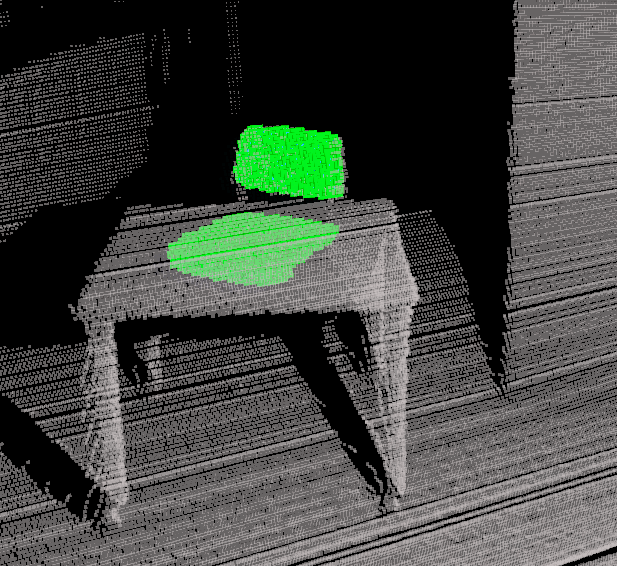
\includegraphics[width=1.6in, height=1.4in]{images/occluded_chair.png}\label{first_scan}}
   \hfil
   \subfigure[Example of a detected table. The detected table model is colored in blue.] {
   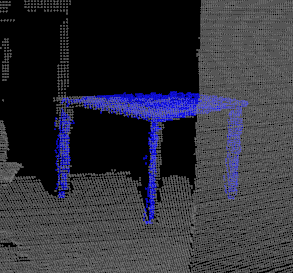
\includegraphics[width=1.6in,height=1.4in]{images/table_behind_wall}}
   \caption{Example of correctly classified furniture. The chair is correctly detected despite the fact that only the top part of the chair is actually visible in the scan. Similarly, the table is detected despite the fact that it is partially occluded.}
   \vspace{-15pt}
   \label{examples}
\end{figure}

Previous work has shown success in classifying mostly unoccluded objects in
different orientations but does not perform well with the
large occlusions typical for human environments. This paper presents the
Verfied Partial Object Detector (VPOD), an algorithm that is capable of
detecting objects despite more than 50\% occlusion. VPOD segments a point
cloud of a scene into clusters by point distances and classifies each resulting cluster. This classification is based on a two step approach. The first step builds upon Viewpoint Feature Histograms (VFH) \cite{Rusu2010}, a descriptor for 3D point cloud data that encodes geometry and viewpoint. The VFH of the query object is computed and compared to VFHs in a database
composed of both complete object models and auto-generated partial object
models. The auto-generated partial models allow for a classification of
parts of an object, whose detection in turn yield a hypothesis of the existence
of the complete objects in the point could. For example, detecting the back of a chair in the
point cloud could indicate the existence of a chair with the
sitting surface occluded by other objects.

However, the existence of partial objects in the database also increases the
risk of false positives. For example, a simple piece of board could be
matched to the back of a chair, leading to a hypothesis of a chair. Our
algorithm therefore introduces a second step to verify each hypothesis. The verification step maps a complete model of the object associated with the candidate match into the point cloud of the scene. Points of the complete model that would be occluded by
objects in the point cloud are then detected and eliminated from the model. The remaining points are checked for matching points in the
point cloud. The proportion of matching, unoccluded points yields the final classification score. 
This steps ensures that matches are consistent with our expectation given the
context of the world and the current viewpoint.

The remainder of this paper will focus on the detection of furniture as a use
case and is organized as follows: Section \ref{relate} discusses related work and Section \ref{vfh} summaries the basic structure of
vanilla VFHs. A detailed analysis of our approach is provided in Section
\ref{analyis} and experimental results are demonstrated in Section
\ref{experiments}. Concluding remarks are given in Section \ref{conclusion}.

%Point Cloud Library (PCL) was used for much of this work.

\section{Related Work}
\label{relate}
The detection of objects in 3D laser data has been studied intensively in
various research fields. As such, we are only addressing the work most relevant
to partial object and furniture detection in human environments.

In \cite{Rusu} Rusu et al. present a system for the acquisition of hybrid Semantic 3D Object Maps for indoor household environments based on 3D point cloud data. The authors use a two step approach for detecting kitchen furniture based on the detection of horizontal and vertical planes as well as knobs.

In \cite{Blodow2007} the authors describe a mapping system acquiring 3D object models for indoor environments. The authors present a system for segmenting and geometrically reconstructing cabinets, tables, drawers and shelves based on multiple scans of the objects. Tables, the most relevant part to our work, are detected by finding horizontal surfaces within a given height range. This does not allow for distinguishing between, for example, tables and shelves.


Holz et al. are using 3D Time-of-Flight cameras in \cite{Holz2010} for semantic scene analysis. The authors are using an MSAC-based approach and surface information in a point's local neighborhood to detect table tops. This is done by assuming that a table top point has a surface normal nearly parallel to the z-axis and that the local surface is smooth. MSAC is used to fit planar surface models into the table point set. This approach yields the same limitations as \cite{Blodow2007}.


Johnson et al. presents in \cite{Johnson2002} a shape-based object recognition system based on matching Spin Images. Spin Images however require a high resolution image, and as such are difficult to use in 3D point clouds obtained by a laser.


Marton et al. incorporate in \cite{Marton} 3D laser scans and 2D vision data for object classification. They use the Radius-based Surface Descriptor (RSD) on 3D data, extract the region of interest into a camera image, and compute a 2D SURF vector for each patch. The final classification is performed through a SVM. However, it remains unclear how this work can be extended to work with furniture, which usually lacks texture. In addition, partial occlusions would be difficult to handle by this approach. % TODO: This should be clarified


Steder et al. \cite{Steder2009} demonstrated the detection of chairs and other objects in 3D point clouds using point features from range images. The authors use euclidean distance in a vector space spanned by Harris feature vectors to find candidates. GOODSAC is used to find a model transformation and false positives are rejected based on a score function using scaled range images. Steder also presented the normal aligned radial features (NARF) in  \cite{Steder2010}. Interest points are detected on stable surface areas with significant local changes. A descriptor is then computed by overlaying a star pattern on the range image generated by looking at the interest point along the estimated normal for this point. The authors also describe the potential of matching the feature descriptors as an object recognition approach. However, we experimented with NARF and found that the descriptor is only of limited use in object recognition due to a lack of local texture in range images and the loss of valuable orientation information during normal alignment. E.g. a horizontal surface becomes indistinguishable from a vertical one.

Mozos et al. \cite{Mozos2011} demonstrate a method of categorizing partially occluded objects from object parts learned from segmented 3D models, which are first segmented based on the object's structure. The database of segmented parts is used to suggest categorizations from a scene. The candidates are combined through Hough voting and verified through model fitting. As this approach segments based on the object's structure, the segmented parts do not correspond exactly with occlusions caused in real scenes, which is a property of the occluding object and the scene, not the occluded object. It remains unclear whether \cite{Mozos2011} is sensitive to partial occlusion of the segmented parts. Our approach segments objects based on common occlusions and relies instead on real 3D scans of objects, which can be generated by the robot, and not prebuilt models.


Viewpoint Feature Histograms as presented by Rusu et al. \cite{Rusu2010} are encoding geometry as well as viewpoint information into a descriptor. The authors demonstrate the effectiveness of the descriptor on a dataset consisting of more than 60 unoccluded kitchenware objects. The first part of VPOD builds upon this work to support partial occlusion and is presented in the following section.


%%%%%%%%%%%%%%%%%%%%%%%%%%%%%%%%%%%%%%%%%%%%%%%%%%%%%%%%%%%%%%%

\section{Viewpoint Feature Histrogram}
\label{vfh}
Viewpoint Feature Histograms are histograms describing the geometrical
relationship between all points in the scan of an object. Rusu et al.
\cite{Rusu2010} show that VFHs can discriminate according to the structure of the entire object, if the entire object is visible.

However the VFH is sensitive to partial occlusions. Consider the scan
visualized in Fig. \ref{first_scan} in which only the top part of the chair is
visible. As the top part of the chair is roughly just a flat surface, the points
have an entirely different geometrical relationship to each other than all the
points for an unoccluded chair. This results in different VFHs for the complete
and partial chair, as shown in Fig. \ref{vfh-diff}. 

\begin{figure}[t]
	\centering 
   \vspace{-10pt}
   \centering
   \includecombinedgraphics[scale=0.75]{images/vfh-diff.tex}
   \vspace{-10pt}
   \caption{Example VFHs for a partial model and its associated complete model.
   The individual components of a VFH can be found in \cite{Rusu2010}.}
   \label{vfh-diff}
   \vspace{-10pt}
\end{figure}

The consequence is that partially occluded objects are not reliably detectable
with VFH or any other method that works with the properties of the complete
object model alone.

%\ldots

%%%%%%%%%%%%%%%%%%%%%%%%%%%%%%%%%%%%%%%%%%%%%%%%%%%%%%%%%%%%%%%


\section{Algorithm}
\label{analyis}

%% This following line wasn't showing up anywhere...
%% In the following discussion, models are simply 3D point clouds of objects at different orientations and distances.
We now outline our approach extending on the use of VFH. 
\subsection{Approach}
The key insight is that fragments of a partially occluded object can be treated
and classified as objects themselves. 
VPOD extends the VFH database to include partial models auto-generated by
occluding portions of complete models. The partial model generation process is
designed to generate typical occlusions occurring in the world. For human environments, we assume that the objects are usually occluded from one side (e.g partially behind a wall) 
or the bottom (e.g. a chair underneath a table). Our algorithm therefore
generates partial models out of every complete model by successively removing
points from each side of the object and from the bottom independently. This is done for a step size $s$ and continued until a threshold $t$ is reached for the remaining 
object size on the side currently affected by the removal. Fig. \ref{diagram}
visualizes an example of this process. Other types of common occlusions can
easily be added by generating additional partial models. The resulting partial models are 
included in the VFH database \emph{with} the complete models.

\begin{figure}[t]
   \vspace{-10pt}
   \centering
   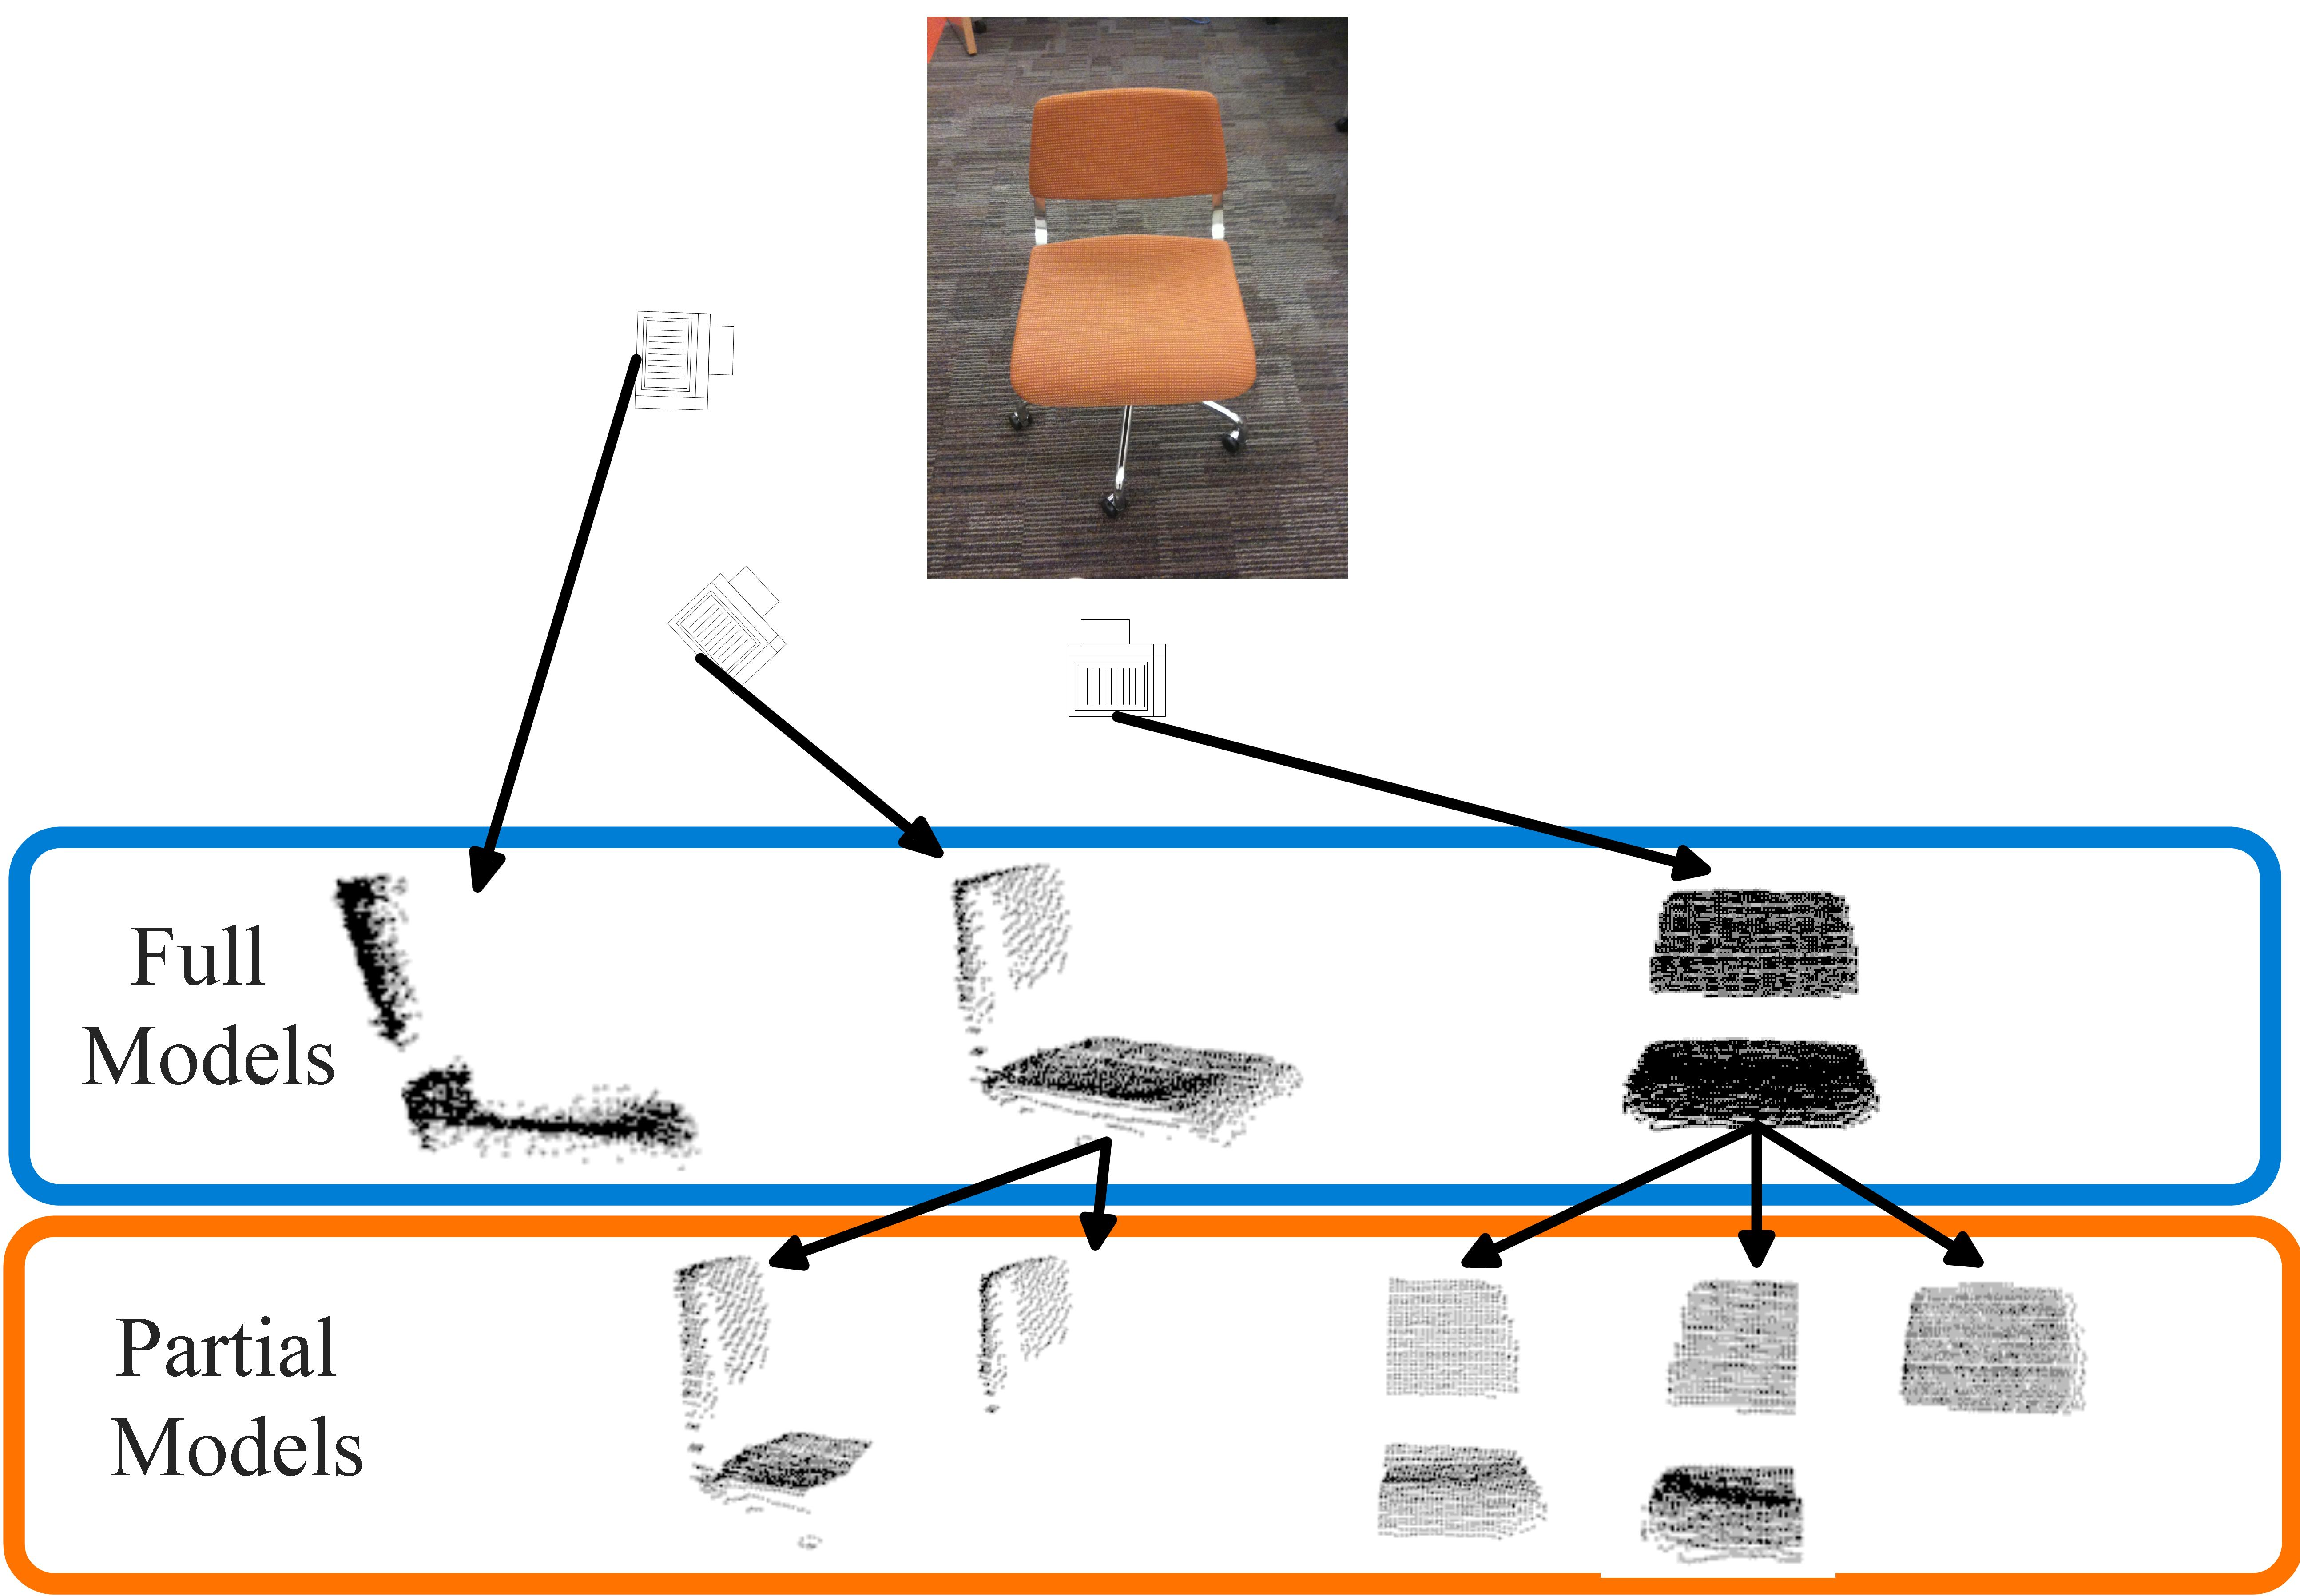
\includegraphics[width=\figw]{images/models.jpeg}
   \vspace{-10pt}
   \caption{Hierarchy of complete models and auto generated partial models.}
   \label{diagram}
   \vspace{-10pt}
\end{figure}

Including partial models in the VFH database increases the likelihood that a partially 
occluded object will be matched. For example, it is now possible to match the back of a 
chair against models in the database that represent just the back of a chair. But this also 
increases the likelihood of false positives, as the partial models are less distinctive 
(e.g. the back of a chair is mostly flat). 
Extending the database to artificially created objects, especially pieces of objects, 
allows for matches of arbitrary objects. To compensate for this, 
the algorithm includes a verification step that verifies the candidate classifications 
against the actual scene in which the point cloud was captured (called the ``world'' from here on).

The intuition behind this verification step is that if the detected part is
indeed a proxy for the actual object in the scene, we can compute our expected
observation for the complete object. This can be done by projecting the complete
object model on the detected part and reasoning about expected occlusions,
which can be determined by a simple line-of-sight test against the scan of the world. The obtained expected
observation can then be matched with the actual observation. For example, if we matched the back of a chair against an object in the world, then the expected observation of the complete chair model projected into the scan has to be
consistent with the world. 

We have implemented this intuition through the following steps:

\begin{enumerate}
  \item the complete model associated with the detected part is mapped into the
  world (section \ref{alignment})
  \item the portions of the complete model expected to be occluded based on
  information provided by the world are removed from the model (section \ref{occlusions})
  \item the remaining model points are checked for matches in the world (section \ref{scoring})
  \item based on this score, the classification is rejected or verified (section
  \ref{scoring})
\end{enumerate}

Fig \ref{uml} summaries the workflow as discussed in
detail in the following.



\begin{figure}[t]
   \vspace{-5pt}
   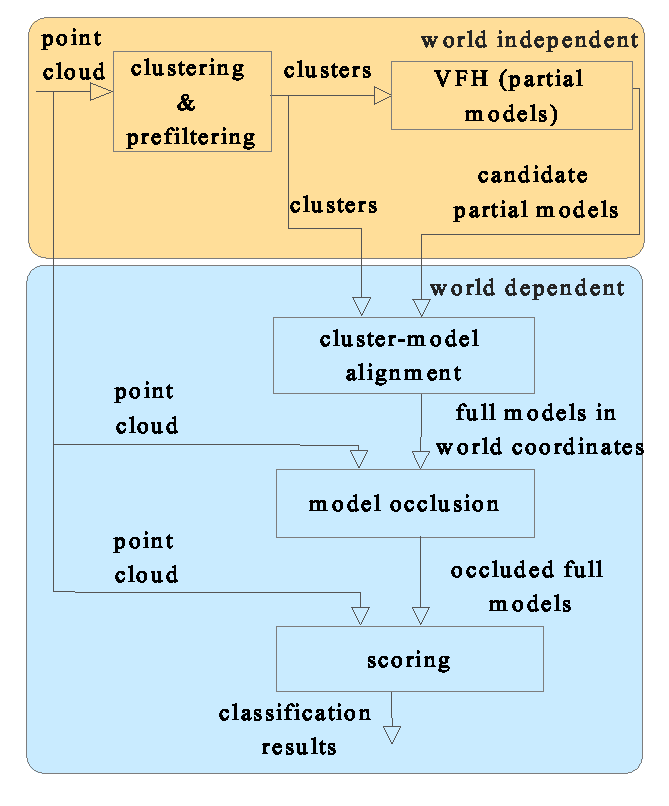
\includegraphics[width=\figw]{images/Concept1.eps}
   \vspace{-15pt}
   \caption{Workflow. Steps independent of the actual world are colored in orange while world dependent steps are colored in blue. }
   \label{uml}
   \vspace{-10pt}
\end{figure}

\subsection{Clustering}
First, the point clouds collected by the robot are segmented into query
clusters. We filter the point cloud to remove outlying points that are not near any surface or object.  
This type of noise is especially common on occlusion boundaries with laser range finders.  
The remaining points are then downsampled to reduce computation time.  
A grid size of 1 cm was used for the downsampling in this work.  
Because the sensor's height relative to the ground is known, we can easily remove the ground plane by 
discarding any points below a given z-coordinate.  
With the ground plane removed, we can then cluster the remaining points. 
 In this work, we require a minimum of 100 points per cluster, and allow 10cm distance between points within a 
 cluster. Objects such as chairs, tables, desks, walls of the room and others
 are returned as clusters. As this work uses furniture as a use case, we
 filtered clusters out that cannot represent furniture or parts of furniture. Filtering was done based on bounding box size and position to
 discard objects that are much too large, much too small, or not near the ground.

\subsection{Alignment}
\label{alignment}
Next, VPOD computes the transformation
matrix $T$ that transforms the centroid of each candidate partial model $M_p$ to
the centroid of the cluster $C$ it was matched against. $T_{center}$ is then
apply to $M_p$. This yields the transformed partial model $M'_p=T_{center} M_p$. 
However, models in a database usually have limited angular resolution, e.g we 
might have a model of a chair rotated at $10^\circ$ and at $20^\circ$ in the database. 
The transformation might not align $M_p$ and $C$ optimally. In order to compensate for this, 
as well as centroid computation errors, Iterative Closet Point (ICP) \cite{ICP} is performed 
on $M'_p$ and $C$. The algorithm assumes that the objects are mostly upright and disqualifies 
candidate models if the rotation around the ground plane is beyond a threshold. 
The resulting transformation matrix $T_{ICP}$ is saved. $T_{center}$ and $T_{ICP}$ are 
now both applied to the complete model $M_c$ out of which $M_p$ was generated
yielding $M'_c=T_{ICP} T_{center} M_c$. Consequently $M'_c$ represents the
complete model $M_c$ mapped into world coordinates at the candidate location.

\subsection{Occlusion}
\label{occlusions}
Each point in the mapped complete model $M'_c$ is now checked for occlusion.
This is done through a technique based on ray casting. We adapted traditional ray
casting to the property of a laser for which the lateral error
typically increases with radial distance. As such, for each point $p$ in $M'_c$,
we check if any point in $W$ lies within a cone originating at the viewpoint origin and facing $p$. 
To check this easily, all the points in $M'_c$ and the world $W$ are transformed to radial coordinates 
around the viewpoint. The slope of the cone is tuned to match the known angular error of the laser. In order to compensate for noise in the radial distance, we require the occluding point to be a minimum distance in front of the occluded point. In addition, because a model should not occlude itself, we remove $C$ from $W$ prior to the occlusion test. Points that have been determined to be occluded in this way are omitted from $M'_c$. The resulting model $M^*_c = {occlude}(M'_c,W)$ is then scored.


\subsection{Scoring}
\label{scoring}
The scoring of $M^*_c$ is done by checking if each point $p$ in $M^*_c$ can be
matched against a point in $W$. A point $p$ in $M^*_c$ is declared to have a
match if $W$ has a point within a small sphere around $p$. The final score is
set to bo the ratio of matched points to total points in $M^*_c$. However,
different scoring techniques are possible here. For example, an additional weighting factor
determined by the number of points in $M^*_c$ could be added to capture the lack of 
evidence that only a small number of points provides. Additionally the scoring
could be done two-ways. This is, ensure that not just $M^*_c$ coincides with $W$
and $C$ but that $C$ also coincides with $M^*_c$. This would guarantee that most points in $C$ have to actually be accounted for. 
Details are discussed in Section \ref{examples}.

%%%%%%%%%%%%%%%%%%%%%%%%%%%%%%%%%%%%%%%%%%%%%%%%%%%%%%%%%%%%%%%

\section{Experiments and Analysis}
\label{experiments}

\begin{figure}[t]
	\centering
	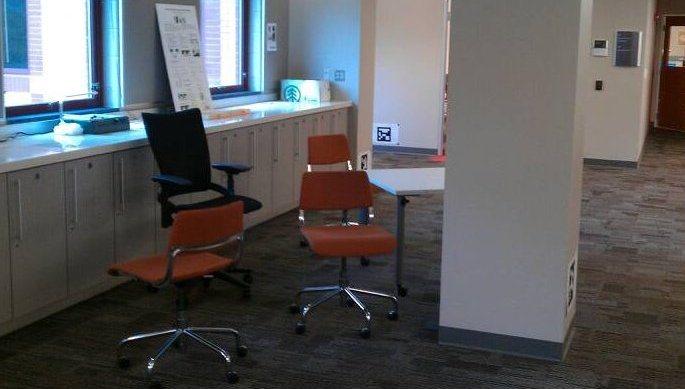
\includegraphics[width=\figw]{images/original_setup4.jpg}
	\vspace{-18pt}
	\caption{Experimental setup.}
	\label{experimental-setup}
\end{figure}
\begin{figure}[t]
	\centering
	\subfigure[Sample point cloud. Red: cluster classified by VFH as the top of a chair.] {
   		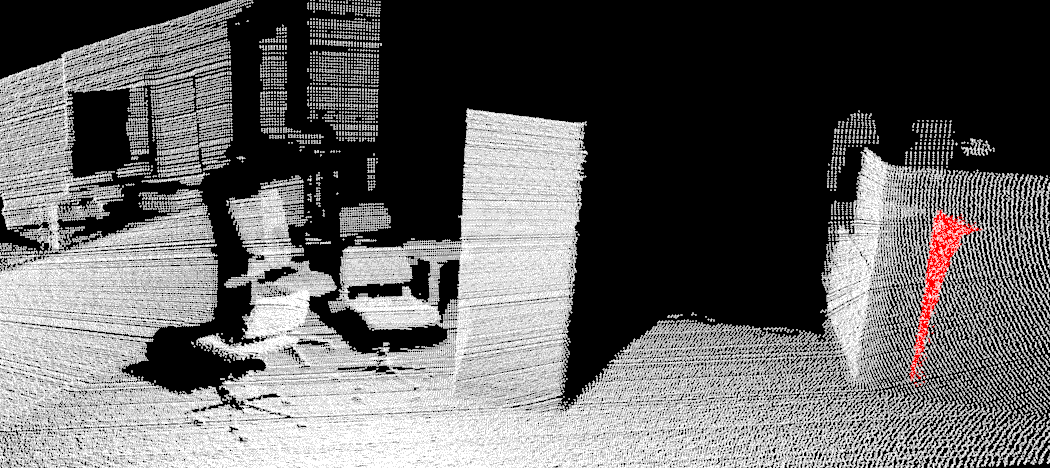
\includegraphics[width=3.3in, height=1.4in]{images/full_cloud_cropped.png}
   		\label{full_cloud}
   	}
	\hfil
	\subfigure[False positive detection.] {
		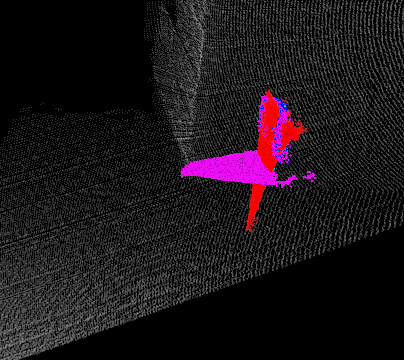
\includegraphics[width=1.58in]{images/chair_in_wall}
		\label{chair_in_wall}
	}
	\subfigure[True positive detection.] {
		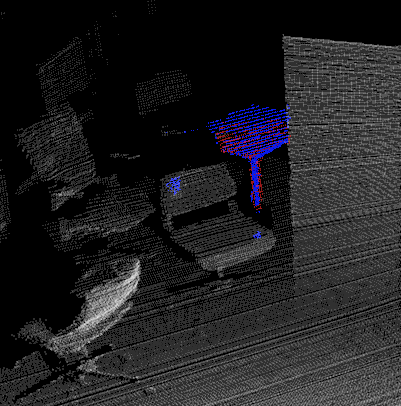
\includegraphics[width=1.58in, height=1.4in]{images/table}
		\label{table_example}
	}
	\vspace{-10pt}
	\caption{Example of false positive and true positive detection.}
	\label{examples}
	\vspace{-15pt}
\end{figure}


To verify our approach, we tested it on real scans obtained through a Hokuyo
laser range finder on a Pan Tilt Unit. 

We first created models of a chair and table for 7 distances and 16 rotations 
from scans with the laser range finder. The distances were chosen to yield a 
constant vertical viewpoint change of 9$^{\circ}$ on the obstacle. For our
sensor height of approximately 1.5m, this resulted in distances of 0.86m, 1.09m, 1.35m, 1.66m, 2.06m, 2.59m and 3.37m. 
For each of the distances, scans of the object with a 22.5$^{\circ}$ 
rotational step size were obtained. This resulted in a total of 224
complete model scans. Out of those models, an additional 1068 partial models
were auto-generated by consecutively removing
points from bottom to top, left to right, and right to left from the model. We used a 10cm step size and proceeded until the remaining model had a size between 20-30cm on the axis currently affected by the point removal. Fig. \ref{diagram} shows an example.

We took 30 test scans of scenes in an office environment with random configurations of up to four 
chairs of different types and two tables per scan. These scenes had non-furniture items, walls, unoccluded
furniture, and partially occluded furniture. For example, some scenes had chairs behind and or pushed under a table. An example setup can be seen in Fig. \ref{experimental-setup} and the
according point cloud is visualized in Fig. \ref{full_cloud}. As shown below,
these are difficult cases for vanilla VFH which uses only complete models.


%\begin{figure}[t]
%\centering
%   \subfigure[Full chair model.] {
%   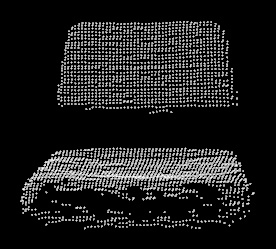
\includegraphics[width=1.25in]{images/full_chair} \label{full_chair}}
%   \hfil
%   \subfigure[Bottom to top cut.] {
%   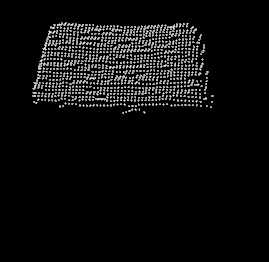
\includegraphics[width=1.16in]{images/chair_top} \label{partway}}
%   \subfigure[Left to right cut. ] {
%   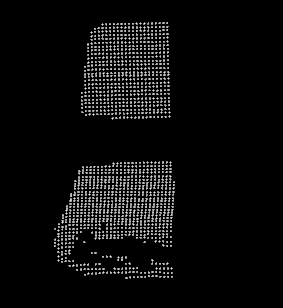
\includegraphics[width=1.25in, height=1.23in]{images/chair_right} \label{full_chair}}
%   \hfil
%   \subfigure[Right to left cut.] {
%   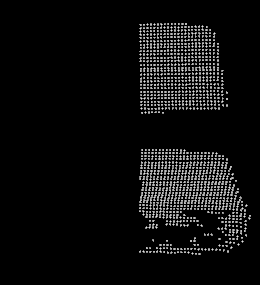
\includegraphics[width=1.2in, height=1.23in]{images/chair_left} \label{partway}}
%\caption{Illustration of partial model creation of a model directly facing the camera.}
%\label{partial_models}
%\vspace{-10pt}
%\end{figure}

\subsection{Results}
To obtain the following results we used the chi-squared distance metric for all
comparisons between VFHs. 

% VPOD was able to accurately classify every
% possible cluster in the test scenes, which included previously unseen furniture types (e.g. Fig \ref{experimental-setup}), with a 3.3\% of the false positives introduced by VFH with full models alone. VFH with full models did not even classify every partially occluded cluster correctly, while providing many false positives.

Fig. \ref{roc-filter}, Fig. \ref{roc-partial}, and Fig. \ref{roc-vpod} visualize
the behavior of the classification error rates of different algorithms as the VFH threshold is relaxed. 
The True Positive Rate (TPR) denotes the ratio of actual furniture correctly
identified; the False Positive Rate (FPR) the ratio of non-furniture incorrectly identified. 
Due to clustering errors explained below, not all objects in all test scenes
could be classified by VFH or VPOD (or could be by any other algorithm that
classifies based on clusters).

\begin{figure}[t]
	\subfigure[Filtering improvement] {
		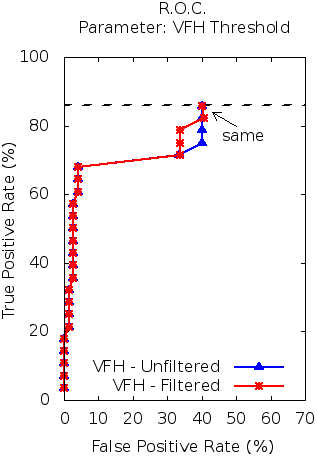
\includegraphics[width=1.575in]{images/filtered-vs-unfiltered.png}
		\label{roc-filter}
	}
	\hfil
	\subfigure[Partial models improvement] {
   		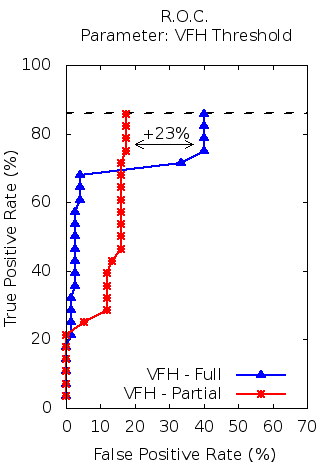
\includegraphics[width=1.575in]{images/partial-vs-full.png}
   		\label{roc-partial}
   	}
	\subfigure[VPOD improvement] {
		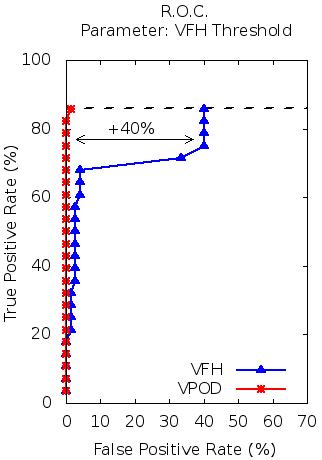
\includegraphics[width=1.6in]{images/vpod-vs-vfh.png}
		\label{roc-vpod}
	}
	\vspace{-5pt}
	\caption{Relative operating characteristic, showing improvement over VFH. Dashed line marks the best possible rate, due to clustering errors.}
	\vspace{-15pt}
\end{figure}

Fig. \ref{roc-filter} shows the behaviour of vanilla VFH using only complete
models on the dataset and the same algorithm with pre-filtering of clusters, as described in Section \ref{clustering}. 
Even if the VFH threshold is relaxed greatly, allowing \emph{many} false
positives, VFH is unable to correctly classify many clusters due to partial
occlusions. Despite having more than 40\% false positive rate, vanilla VFH was
not able to achieve the maximal possible classification rate on our dataset. Even at a low threshold,
 vanilla VFH still produced a 5\% false positive rate while only
classifying 70\%. Prefiltering provides only a modest reduction in the false positives produced by VFH. 
This sows that pre-filtering alone does not account for all of the benefits of
VPOD.

Fig. \ref{roc-partial} shows the behaviour of VFH with and without partial models. 
At very low VFH thresholds, the partial models have no effect. 
As the threshold increases, the partial models are allowed to incorrectly match clusters, 
causing an increase in the false positive rate relative to complete models
alone. But vanilla VFH using only complete models can only match the unoccluded
clusters well and must allow many false positives in order to match the partially occluded clusters. However, VFH with partial models is able to classify all test clusters with a 23 point reduction in the FPR. This is because VFH with partial models can match partially occluded clusters using a tighter VFH threshold.

Fig. \ref{roc-vpod} shows the behaviour of VPOD compared to VFH using complete
models. Fig. \ref{roc-vpod} shows that VPOD, through the use of partial models,
similar to Fig. \ref{roc-partial}, properly classified \emph{all} test
cases. Unlike VFH with partial models, VPOD classified all test cases with only a 1.3\% false positive rate, due to the VPOD verification step. This allows VPOD to classify the partially occluded objects without introducing many false positives.

These results demonstrate the usefulness of VPOD.
\subsection{Examples}
\label{examples}
We disabled the pre-filtering and ICP restriction on y-axis rotation to obtain the following examples.

Fig. \ref{chair_in_wall} demonstrates an example of the false positive
detection. VFH classification with partial models classified the cluster marked red in Fig. \ref{full_cloud} 
as being the top part of a chair. The algorithm then mapped the complete chair
into world and scored it. Since the sitting surface is not occluded but also not visible in the scan this classification was rejected. 
In contrast, the table behind the chairs in Fig. \ref{full_cloud} was matched by VFH with partial models and verified 
by the algorithm. Note that due to the occlusion, vanilla VFH using just
complete models would not be able to classify the table.

Fig. \ref{counter_example} demonstrates a typical example where our algorithm fails if no pre-filtering or two-way matching is performed. If the cluster is unreasonably large, almost any furniture piece can be fitted in and have its points being accounted for. In Fig. \ref{counter_example} a chair (green) is being fitted into a big wall (fitted chair shown in blue). The algorithm is effectively saying that the chair is lodged in the wall. This demonstrates the necessity of pre-filtering or two-way matching in combination with our algorithm.

\vspace{-5pt}
\subsection{Clustering}
\label{clustering}

\begin{figure}[t]
\centering
   \subfigure[Example of a chair and table being clustered together.] {
   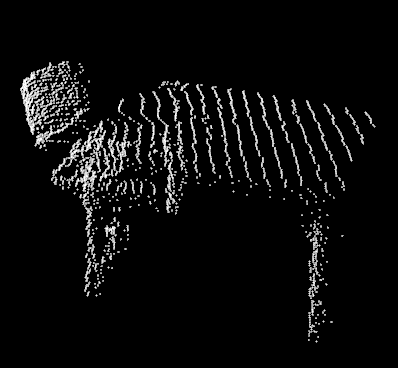
\includegraphics[width=1.55in, height=1.30in]{images/table+chair.png} \label{multiple_cluster}}
   \subfigure[Example of a small model fitted into a big cluster.] {
   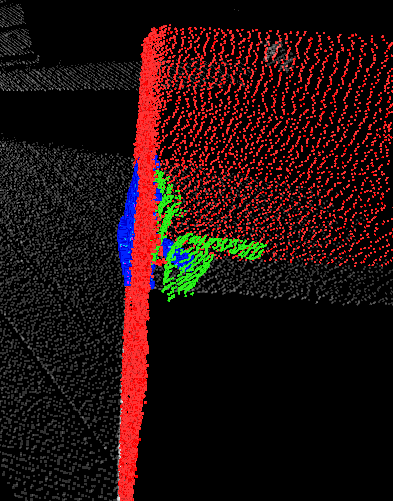
\includegraphics[width=1.55in, height=1.30in]{images/counter_example.png} \label{counter_example}}
   \hfil
\caption{Examples of where our algorithm fails.}
\label{partial_models}
\vspace{-15pt}
\end{figure}


The clustering distance is currently set to a fixed value. This can yield results similar to Fig. \ref{multiple_cluster} where multiple furniture pieces have been clustered together, which hinders classification. In future work we plan to have the clustering distance be data driven. The basic assumption is that points on the same object have a smaller relative distance to each other than points between objects. We therefore plan to evaluate the distances of points within a cluster and re-cluster a cluster based on a new, smaller distance. Clusters that are not classified can be progressively partitioned and reclassified until either a match is found or the cluster size is unreasonably small.

Further, many objects such as chairs and tables can appear as multiple distinct parts due to self-occlusions.  For example, when observing most standard office chairs, we typically observe the chair's seat, back, and wheeled base, but not the central supporting column due to the downward viewing angle. Similar results can occur as well with other types of furniture.  To address this problem, we plan to project the clusters down to the ground plane, find the convex hull for each, and merge clusters that have overlap.  This allows us to consider such objects as one unit, despite being separated by a significant vertical distance. Again, this step can be verified by checking if the classification results have improved in comparison to the single clusters.

\vspace{-5pt}
\subsection{Runtime}
We are performing the occlusion and matching simultaneously in VPOD. 
As such the occlusion and matching together takes an average of 3.3 seconds for a world scan with about 
32,000 points and an average cluster size of 19,000 points. If runtime is a concern the 
occluding and matching do not need to be run against the full point cloud. Rather, 
it can easily be determined which parts of the world are affecting the current occlusion 
and matching operation and the operation be performed against a subset of the world. 
%The additional runtime can be justified in domains that call for the greater
%classification accuracy provided.

%%%%%%%%%%%%%%%%%%%%%%%%%%%%%%%%%%%%%%%%%%%%%%%%%%%%%%%%%%%%%%%


\section{Conclusion}
\label{conclusion}

In this paper we presented the VPOD algorithm for detecting partially occluded objects by 
matching clusters against segments of models and verifying our expectations against the world. 
VPOD extends the scope of vanilla VFH classification by using
partial models. To reject false positives, VPOD verifies expectations about the predicted classification 
with the world. We verified the effectiveness of our approach on real data, showing 
improvement on cases not handled by VFH with complete models alone.

We are currently working on improving the clustering algorithm as described above. In addition, we are investigating techniques of enhancing the clustering through feedback from the algorithm. It is possible to eliminate points from a cluster which correspond with points in a matching model and rerun the remaining cluster. For example the cluster visualized in Fig. \ref{multiple_cluster} was actually classified as a table by our algorithm, the table could then be removed from the cluster and the remaining cluster classified as a chair.

Further, we are currently integrating VPOD into semantic mapping and NAMO
algorithms on our robot.

\section*{Acknowledgments}
ROS was used for most parts of this work. This research was supported by NSF
grant IIS-1017076.

%%%%%%%%%%%%%%%%%%%%%%%%%%%%%%%%%%%%%%%%%%%%%%%%%%%%%%%%%%%%%%%

\bibliographystyle{plain}
\bibliography{furniture}

\end{document}


